\documentclass[main.tex]{subfiles}

\begin{document}
%-------------------------------------------------------------------------------
%---------------------------------- Section 2 ----------------------------------
%-------------------------------------------------------------------------------
\section{Differenciálegyenletek}

%-------------------------------------------------------------------------------
%-------------------------------- Subsection 2.1 -------------------------------
%-------------------------------------------------------------------------------
\subsection{Bevezetés}

\defi{0}{.33}{Differenciálegyenlet}

! $y : \mathbb{R} \rightarrow \mathbb{R}$ $n$-szer
folytonosan differenciálható függvény, vagyis
$y^{(0)} = y;\; y^{(1)} = y';\; y^{(2)} = y'';\; \dots \; ;\;  y^{(n)}$
folytonos fóggvények, $x$ független változó. Ekkor az
$F \left( x ; y ; y' ; \dots ; y^{(n)} \right)$
egyenletet $y$-ra vonatkoztatott, $n$-edrendű,
közönséges differenciálegyenletnek nevezzük.



\megj{1}{0}
\begin{itemize}
  \item A közönséges arra utal, hogy egy
        független változót tartalmaz az egyenlet.
        Ha nem közönséges, akkor parciális
        (többváltozós) a diffegyenlet.

  \item A rend a legmagasabb fokú deriváltra utal.
\end{itemize}



\pelda{1}{8}



\defi{1}{.33}

Azt a differenciálegyenletet, amelyben az ismeretlen
függvény, és annak deriváltjai csak elsőfokon,
szorzatuk pedig egyáltalán nem fordul elő,
lineáris diffegyenletnek mondjuk. Ellenkező
esetben nemlineáris.



\megj{1}{0}

\begin{itemize}
  \item $F \left( x ; y ; y' ; \dots ; y^{(n)} \right) = 0$
        \tabto{4.9cm} – \tabto{5.5cm} implicit megadás

  \item $y^{(n)} = \left( x ; y ; y' ; \dots ; y^{(n-1)} \right)$
        \tabto{4.9cm} – \tabto{5.5cm} explicit megadás
\end{itemize}



\defi{1}{.33}

Az $F \left( x ; y ; y' ; \dots ; y^{(n)} \right) = 0$
diffegyenlet megoldása a
$\varphi : \mathbb{R} \rightarrow \mathbb{R}$
függvény, ha $\forall x \in \mathbb{R}$-re teljesül
\begin{equation*}
  F \left( x ; \varphi(x) ; \varphi'(x) ; \dots ; \varphi(x)^{(n)} \right) = 0.
\end{equation*}



\pelda{0}{14}



\defi{1}{.33}

A közönséges differenciálegyenlet megoldásfüggvényének
görbéje a differenciálegyenlet integrálgörbéje/megoldásgörbéje.




\defi{1}{.33}{Általános megoldás}

Azt a megoldást, ami azonosan kiegészíti a diffegyenletet,
és pontosan annyi egymástól független állandót tartalmaz,
ahányad rendű a differenciálegyenlet, általános megoldásnak
nevezzük.




\defi{1}{.33}{Partikuláris megoldás}

Azt a megoldást, amely az általános megoldásból úgy származtatható,
hogy az abban szereplő konstansoknak meghatározott értéket adunk,
partikuláris megoldásnak nevezzük.

\vspace{.33em}
Általánosabban partikuláris megoldásról beszélünk, ha a
megoldásfüggvény legalább eggyel kevesebb egymástól
független konstanst tartalmaz, mint ahányad rendű az egyenlet.




\defi{1}{.33}{Szinguláris megoldás}

A szinguláris megoldás olyan megoldás,
amely nem kapható meg az általános megoldásból
a konstansok megfelelő megválasztásával.



\pelda{1}{.33}

\begin{minipage}[c]{.4\textwidth}
  \begin{figure}[H]
    \centering
    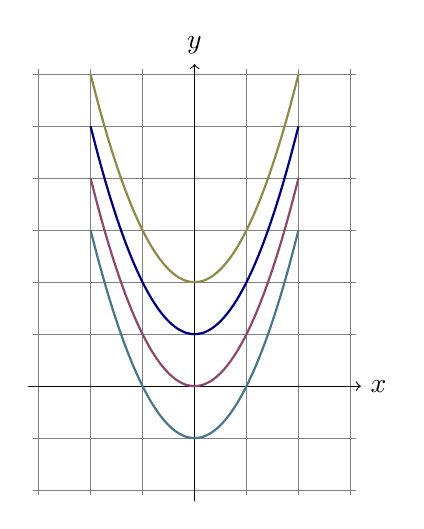
\begin{tikzpicture}[scale = .66]
      \draw[very thin,color=gray] (-3.1,-2.1) grid (3.1,6.1);
      \draw[->] (-3.2,0) -- (3.2,0) node[right] {$x$};
      \draw[->] (0,-2.2) -- (0,6.2) node[above] {$y$};

      \draw[thick, magenta!50!black ,domain=-2:2, smooth] plot ({\x},{\x*\x});
      \draw[thick, blue!50!black    ,domain=-2:2, smooth] plot ({\x},{\x*\x + 1});
      \draw[thick, yellow!50!black  ,domain=-2:2, smooth] plot ({\x},{\x*\x + 2});
      \draw[thick, cyan!50!black    ,domain=-2:2, smooth] plot ({\x},{\x*\x - 1});
    \end{tikzpicture}

    \caption{$y = x^2 + C$}
  \end{figure}
\end{minipage}\hfill
\begin{minipage}[c]{.6\textwidth}
  Keressünk az $y' = 2x$ differenciálegyenletnek olyan megoldását,
  melyre teljesül, hogy $y(1) = 4$.
  \begin{align*}
    \hspace{5em} y' & = 2x      &  & {/\textstyle\int \, \differential x}
    \\
    y               & = x^2 + C
    \\
  \end{align*}
  Tudjuk, hogy a megoldásgörbe átmegy az $(1; 4)$ ponton:
  \begin{align*}
    y(1) & = 1^2 + C = 4 \\
    C    & = 3           \\
    y    & = x^2 + 3
  \end{align*}
\end{minipage}



\defi{1}{.33}{Cauchy-feladat}

Ha az $n$-ed rendű differenciálegyenlet olyan megoldását
keressük, hogy
\begin{equation*}
  y(x_0) = y_0, \quad
  y'(x_0) = y_0', \quad
  y''(x_0) = y_0'', \quad
  \dots, \quad
  y^{(n)}(x_0) = y_0^{(n)}
\end{equation*}
feltételeket kiegyenlíti, akkor Cauchy-feladatról,
vagyis kezdeti éték feladatról beszélünk.



\megj{1}{.33}

A Cauchy-feladat megoldása a differenciálegyenlet
partikuláris megoldása. Elsőrendű diffegyenlet
esetén ez azt jelenti, hogy Keressük az
$(x_0; y_0)$ ponton átmenő integrálgörbét.

\vspace{.33em}
Differenciálegyenlet megoldása esetén arra a kérdésre
kell válaszolnunk, hogy milyen feltételek mellett
van az egyenletnek megoldása, egyértelmű megoldása,
és ezek hogyan érhetőek el.












\end{document}